\documentclass[a4paper,11pt]{article}
\input{/home/tof/Documents/Cozy/latex-include/preambule_doc.tex}
\input{/home/tof/Documents/Cozy/latex-include/preambule_commun.tex}
\newcommand{\showprof}{show them}  % comment this line if you don't want to see todo environment
\setlength{\fboxrule}{0.8pt}
\fancyhead[L]{\fbox{\Large{\textbf{Algo 15}}}}
\fancyhead[C]{\textbf{Exercices représentation}}
\newdate{madate}{10}{09}{2020}
%\fancyhead[R]{\displaydate{madate}} %\today
\fancyhead[R]{Terminale - NSI}
\fancyfoot[L]{\vspace{1mm}Christophe Viroulaud}
\AtEndDocument{\label{lastpage}}
\fancyfoot[C]{\textbf{Page \thepage/\pageref{lastpage}}}
\fancyfoot[R]{\includegraphics[width=2cm,align=t]{/home/tof/Documents/Cozy/latex-include/cc.png}}

\begin{document}
\begin{exo}
    Dessiner tous les graphes non orientés ayant exactement trois sommets.
\end{exo}
\begin{exo}
    \begin{center}
        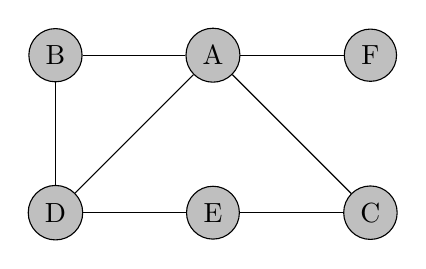
\begin{tikzpicture}
            \node[draw,circle,fill=gray!50] (A)at(0,2) {A};
            \node[draw,circle,fill=gray!50] (B)at(-2,2) {B};
            \node[draw,circle,fill=gray!50] (C)at(2,0) {C};
            \node[draw,circle,fill=gray!50] (D)at(-2,0) {D};
            \node[draw,circle,fill=gray!50] (E)at(0,0) {E};
            \node[draw,circle,fill=gray!50] (F)at(2,2) {F};
            \draw[-,>=latex] (A) -- (B);
            \draw[-,>=latex] (A) -- (C);
            \draw[-,>=latex] (A) -- (D);
            \draw[-,>=latex] (D) -- (B);
            \draw[-,>=latex] (D) -- (E);
            \draw[-,>=latex] (C) -- (E);
            \draw[-,>=latex] (F) -- (A);

        \end{tikzpicture}
    \end{center}
    \begin{enumerate}
        \item Calculer le degré de chaque nœud.
        \item Calculer la somme des degrés.
        \item Construire la matrice d'adjacence (sur papier puis sur machine) du graphe.
        \item Construire le dictionnaire d'adjacence du graphe.
    \end{enumerate}
\end{exo}
\begin{exo}
    \begin{center}
        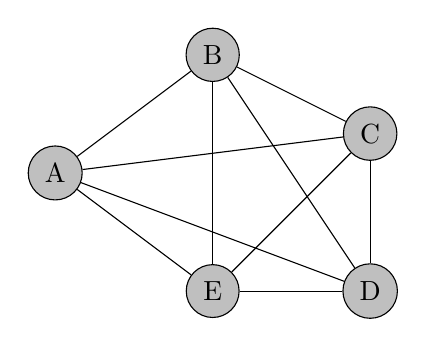
\begin{tikzpicture}
            \node[draw,circle,fill=gray!50] (A)at(-2,1.5) {A};
            \node[draw,circle,fill=gray!50] (B)at(0,3) {B};
            \node[draw,circle,fill=gray!50] (C)at(2,2) {C};
            \node[draw,circle,fill=gray!50] (D)at(2,0) {D};
            \node[draw,circle,fill=gray!50] (E)at(0,0) {E};

            \draw[-,>=latex] (A) -- (B);
            \draw[-,>=latex] (A) -- (C);
            \draw[-,>=latex] (A) -- (D);
            \draw[-,>=latex] (B) -- (D);
            \draw[-,>=latex] (B) -- (C);
            \draw[-,>=latex] (C) -- (D);
            \draw[-,>=latex] (A) -- (E);
            \draw[-,>=latex] (E) -- (D);
            \draw[-,>=latex] (C) -- (E);
            \draw[-,>=latex] (E) -- (B);

        \end{tikzpicture}
    \end{center}
    \begin{enumerate}
        \item Le graphe est-il complet?
        \item Construire la matrice d'adjacence du graphe.
        \item Écrire la fonction \textbf{\texttt{ordre(mat: list) $\rightarrow$ int}} qui renvoie l'ordre du graphe.
        \item Écrire la fonction \textbf{\texttt{est\_complet(mat:list) $\rightarrow$ bool}} qui renvoie \textbf{\texttt{True}} si le graphe st complet.
    \end{enumerate}
\end{exo}
\begin{exo}
    \begin{center}
        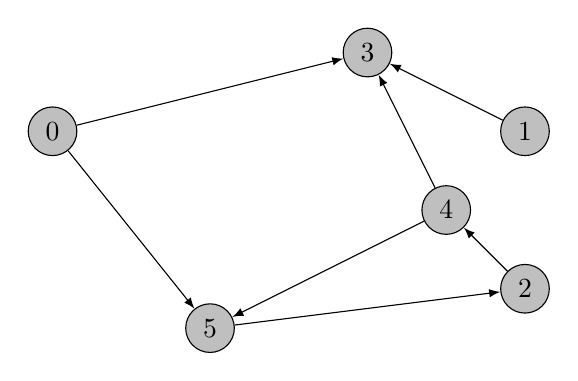
\begin{tikzpicture}
            \node[draw,circle,fill=gray!50] (A)at(-4,2) {0};
            \node[draw,circle,fill=gray!50] (B)at(2,2) {1};
            \node[draw,circle,fill=gray!50] (C)at(2,0) {2};
            \node[draw,circle,fill=gray!50] (D)at(0,3) {3};
            \node[draw,circle,fill=gray!50] (E)at(1,1) {4};
            \node[draw,circle,fill=gray!50] (F)at(-2,-.5) {5};
            \draw[->,>=latex] (F) -- (C);
            \draw[->,>=latex] (A) -- (D);
            \draw[<-,>=latex] (D) -- (B);
            \draw[<-,>=latex] (D) -- (E);
            \draw[->,>=latex] (C) -- (E);
            \draw[<-,>=latex] (F) -- (A);
            \draw[<-,>=latex] (F) -- (E);
        \end{tikzpicture}
    \end{center}
    \begin{enumerate}
        \item Calculer les degrés entrants et sortants de chaque nœud.
        \item Calculer la somme des degrés.
        \item Construire la matrice des successeurs du graphe.
        \item Dans le cas d'un graphe dont les sommets sont numérotés de 0 à \emph{n}, on peut construire une liste d'adjacence où les indices de la liste correspondent aux numéros des sommets. Construire la liste \textbf{\texttt{suivants}} des successeurs du graphe.
        \item Écrire la fonction \textbf{\texttt{degres\_sortants(liste: list, s: int) $\rightarrow$ int}} qui renvoie la valeur du degré sortant de \textbf{\texttt{s}}.
        \item Écrire la fonction \textbf{\texttt{degres\_entrants(liste: list, s: int) $\rightarrow$ int}} qui renvoie la valeur du degré entrant de \textbf{\texttt{s}};
    \end{enumerate}
\end{exo}
\end{document}